\documentclass{standalone}
\usepackage[T1]{fontenc}
\usepackage{amsmath,amssymb}
\usepackage{pgfplots}

\begin{document}
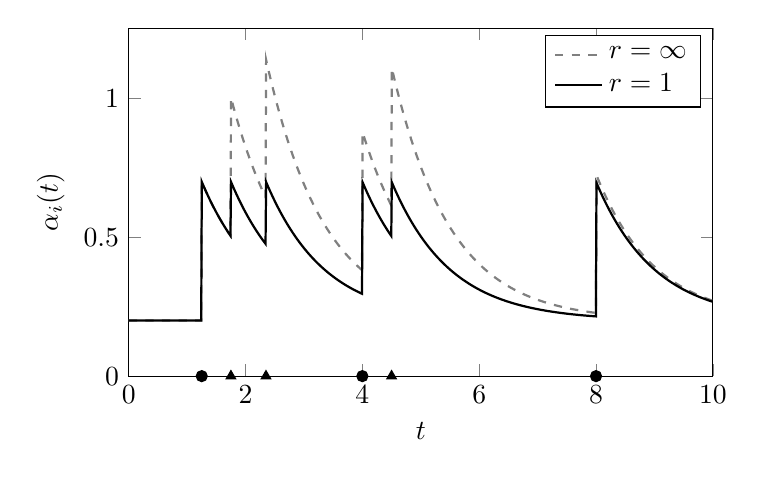
\begin{tikzpicture}
\begin{axis}[xmin=0,xmax=10,ymin=0,xlabel=$t$,ylabel=$\alpha_i(t)$,height=6cm,width=9cm, legend cell align={left}]
	
	%% Define parameters for alpha
	\def\thetaa{0.5}
	\def\gammaa{1}
	\def\lama{0.2}
	
	\addplot[domain=0:10, samples=1000, style=thick, dashed, gray] {(\lama + 
	(x > 1.25 ? \thetaa*exp(-\gammaa*(x-1.25)) : 0) + 
	(x > 1.75 ? \thetaa*exp(-\gammaa*(x-1.75)) : 0) + 
	(x > 2.35 ? \thetaa*exp(-\gammaa*(x-2.35)) : 0) + 
	(x > 4.0 ? \thetaa*exp(-\gammaa*(x-4.0)) : 0) + 
	(x > 4.5 ? \thetaa*exp(-\gammaa*(x-4.5)) : 0) + 
	(x > 8 ? \thetaa*exp(-\gammaa*(x-8)) : 0) 
	)};
	\addlegendentry{$r=\infty$};

	\addplot[domain=0:10, samples=1000, style=thick] {(\lama + 
	(x > 1.25 ? \thetaa*exp(-\gammaa*(x-1.25)) : 0) + 
	(x > 1.75 ? \thetaa*exp(-\gammaa*(x-1.75))-\thetaa*exp(-\gammaa*(x-1.25)) : 0) + 
	(x > 2.35 ? \thetaa*exp(-\gammaa*(x-2.35))-\thetaa*exp(-\gammaa*(x-1.75)) : 0) + 
	(x > 4.0 ? \thetaa*exp(-\gammaa*(x-4.0))-\thetaa*exp(-\gammaa*(x-2.35)) : 0) + 
	(x > 4.5 ? \thetaa*exp(-\gammaa*(x-4.5))-\thetaa*exp(-\gammaa*(x-4.0)) : 0) + 
	(x > 8 ? \thetaa*exp(-\gammaa*(x-8))-\thetaa*exp(-\gammaa*(x-4.5)) : 0)
	)};
	\addlegendentry{$r=1$};
	
	\addplot[mark=*] coordinates {(1.25,0)};
	\addplot[mark=triangle*] coordinates {(1.75,0)};
	\addplot[mark=triangle*] coordinates {(2.35,0)};
	\addplot[mark=*] coordinates {(4.0,0)};
	\addplot[mark=triangle*] coordinates {(4.5,0)};
	\addplot[mark=*] coordinates {(8,0)};

\end{axis}
\end{tikzpicture}
\end{document}
